\documentclass[10pt]{article}
\usepackage[utf8]{inputenc}
\usepackage[T1]{fontenc}
\usepackage{amsmath}
\usepackage{amsfonts}
\usepackage{amssymb}
\usepackage{stmaryrd}
\usepackage{hyperref}
\hypersetup{colorlinks=true, linkcolor=blue, filecolor=magenta, urlcolor=cyan,}
\urlstyle{same}
\usepackage{graphicx}
\usepackage[export]{adjustbox}
\usepackage{mdframed}
\usepackage{booktabs,array,multirow}
\usepackage{esint}
\usepackage{xeCJK}
\usepackage{adjustbox}
\newcommand{\HRule}{\begin{center}\rule{0.5\linewidth}{0.2mm}\end{center}}
\graphicspath{ {./images/} }
\begin{document}

\section*{知识板块二 原电池}

\section*{【知识模块 1】原电池}

\begin{itemize}
\item 原电池的定义: 将化学能转化为电能的装置, 本质为自发进行的氧化还原反应。
\end{itemize}

\section*{原电池的构成条件}

1、活性不同的两极 2、自发的氧化还原反应

3、闭合回路 4、电解质

【思考 1】以下装置能构成原电池吗? 完成以下问题。

\begin{center}
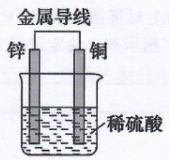
\includegraphics[max width=0.2\textwidth]{images/0190d978-baee-71c0-9ae7-986c76919c41_0_416326.jpg}
\end{center}

\begin{itemize}
\item 电极方程式:
\end{itemize}

①正极: 反应类型:

②负极: 反应类型:

总反应方程式:

\begin{itemize}
\item 电路 (电子不下水, 离子不上岸)
\end{itemize}

1、电流流向:

2、电子流向:

3、离子流向:

【思考 2】以下装置能形成原电池吗?

\begin{center}
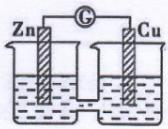
\includegraphics[max width=0.2\textwidth]{images/0190d978-baee-71c0-9ae7-986c76919c41_0_323382.jpg}
\end{center}

硫酸

\begin{center}
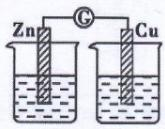
\includegraphics[max width=0.2\textwidth]{images/0190d978-baee-71c0-9ae7-986c76919c41_0_740902.jpg}
\end{center}

硫酸 B

\begin{center}
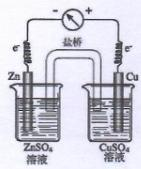
\includegraphics[max width=0.2\textwidth]{images/0190d978-baee-71c0-9ae7-986c76919c41_0_865857.jpg}
\end{center}

A

\end{document}